\documentclass[border=10pt]{standalone}
\usepackage{pgfplots}
\usetikzlibrary{arrows.meta}
\pgfplotsset{compat=1.18, trig format plots=deg}
\begin{document}
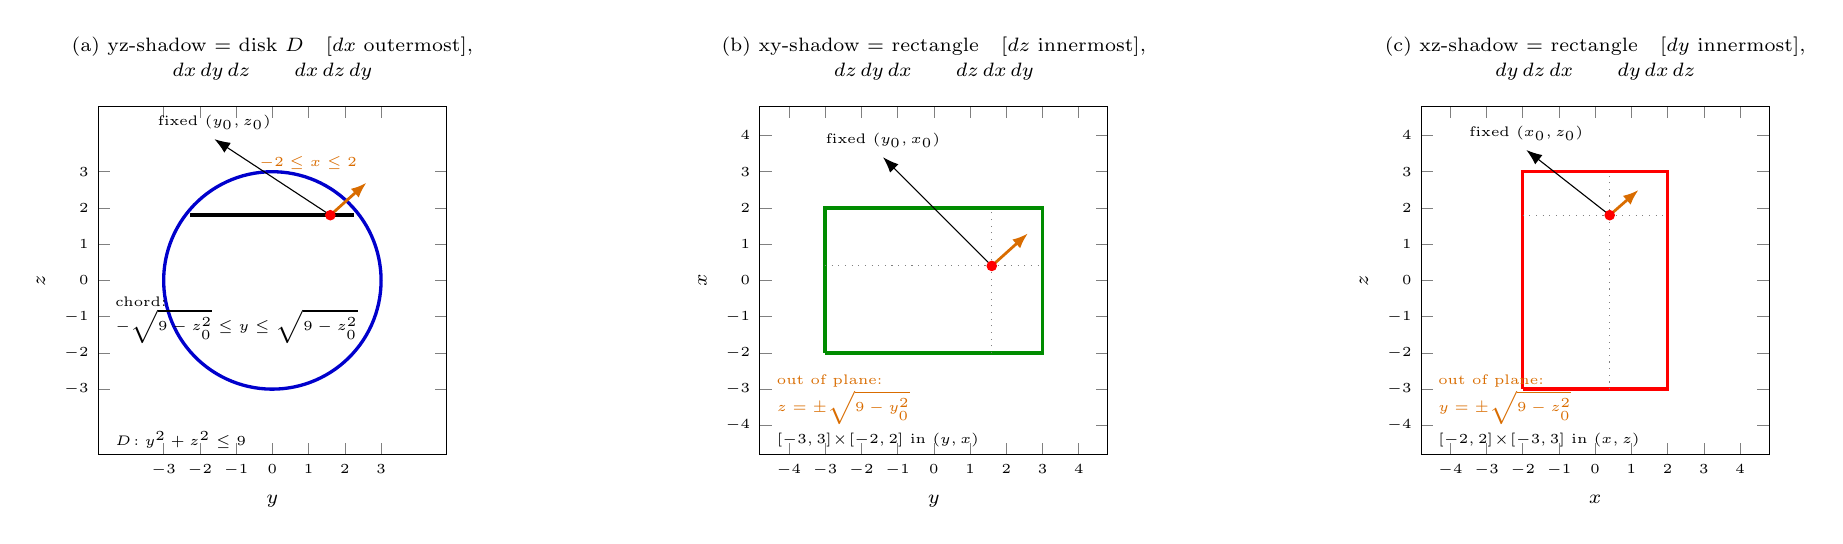
\begin{tikzpicture}[font=\scriptsize]

% ================= (a) yz-shadow : the disk =================
\begin{axis}[
  at={(0,0)}, width=6.0cm, height=6.0cm, axis equal,
  xmin=-4.8, xmax=4.8, ymin=-4.8, ymax=4.8,
  xtick={-3,...,3}, ytick={-3,...,3},
  xlabel=$y$, ylabel=$z$,
  tick label style={font=\tiny}, label style={font=\scriptsize},
  title={(a) yz-shadow $=$ disk $D$\quad [$dx$ outermost],\\[1pt]
         $\displaystyle dx\,dy\,dz\qquad dx\,dz\,dy$},
  title style={font=\scriptsize, align=center},
]
\addplot[blue!30!white, opacity=0.4, draw=none, domain=0:360, samples=120] ({3*cos(x)},{3*sin(x)});
\addplot[blue!80!black, very thick, domain=0:360, samples=120] ({3*cos(x)},{3*sin(x)});
\addplot[black, line width=1.4pt] coordinates {(-2.265,1.8) (2.265,1.8)};
\addplot[only marks, mark=*, mark size=1.7pt, red] coordinates {(1.6,1.8)};
\draw[-{Latex[length=2mm]}, black] (axis cs:1.6,1.8) -- (axis cs:-1.6,3.9);
\node[font=\tiny, anchor=south] at (axis cs:-1.6,3.9) {fixed $(y_0,z_0)$};
\draw[-{Latex[length=2mm]}, orange!85!black, line width=1pt] (axis cs:1.6,1.8) -- (axis cs:2.6,2.7);
\node[font=\tiny, orange!85!black, anchor=south east] at (axis cs:2.6,2.8) {$-2\le x\le 2$};
\node[font=\tiny, anchor=west, align=left] at (axis cs:-4.6,-1.1) {chord:\\ $-\sqrt{9-z_0^{2}}\le y\le\sqrt{9-z_0^{2}}$};
\node[font=\tiny, anchor=west] at (axis cs:-4.6,-4.4) {$D\!: y^{2}+z^{2}\le 9$};
\end{axis}

% ================= (b) xy-shadow : rectangle =================
\begin{axis}[
  at={(8.4cm,0)}, width=6.0cm, height=6.0cm, axis equal,
  xmin=-4.8, xmax=4.8, ymin=-4.8, ymax=4.8,
  xtick={-4,...,4}, ytick={-4,...,4},
  xlabel=$y$, ylabel=$x$,
  tick label style={font=\tiny}, label style={font=\scriptsize},
  title={(b) xy-shadow $=$ rectangle\quad [$dz$ innermost],\\[1pt]
         $\displaystyle dz\,dy\,dx\qquad dz\,dx\,dy$},
  title style={font=\scriptsize, align=center},
]
\addplot[green!35!black!40!white, opacity=0.3, draw=none] coordinates {(-3,-2) (3,-2) (3,2) (-3,2)};
\addplot[green!55!black, very thick] coordinates {(-3,-2) (3,-2) (3,2) (-3,2) (-3,-2)};
\addplot[gray, dotted, thin] coordinates {(-3,0.4) (3,0.4)};
\addplot[gray, dotted, thin] coordinates {(1.6,-2) (1.6,2)};
\addplot[only marks, mark=*, mark size=1.7pt, red] coordinates {(1.6,0.4)};
\draw[-{Latex[length=2mm]}, black] (axis cs:1.6,0.4) -- (axis cs:-1.4,3.4);
\node[font=\tiny, anchor=south] at (axis cs:-1.4,3.4) {fixed $(y_0,x_0)$};
\draw[-{Latex[length=2mm]}, orange!85!black, line width=1pt] (axis cs:1.6,0.4) -- (axis cs:2.6,1.3);
\node[font=\tiny, orange!85!black, anchor=west, align=left] at (axis cs:-4.6,-3.3) {out of plane:\\ $z=\pm\sqrt{9-y_0^{2}}$};
\node[font=\tiny, anchor=west] at (axis cs:-4.6,-4.4) {$[-3,3]\!\times\![-2,2]$ in $(y,x)$};
\end{axis}

% ================= (c) xz-shadow : rectangle =================
\begin{axis}[
  at={(16.8cm,0)}, width=6.0cm, height=6.0cm, axis equal,
  xmin=-4.8, xmax=4.8, ymin=-4.8, ymax=4.8,
  xtick={-4,...,4}, ytick={-4,...,4},
  xlabel=$x$, ylabel=$z$,
  tick label style={font=\tiny}, label style={font=\scriptsize},
  title={(c) xz-shadow $=$ rectangle\quad [$dy$ innermost],\\[1pt]
         $\displaystyle dy\,dz\,dx\qquad dy\,dx\,dz$},
  title style={font=\scriptsize, align=center},
]
\addplot[red!40!white, opacity=0.3, draw=none] coordinates {(-2,-3) (2,-3) (2,3) (-2,3)};
\addplot[red, very thick] coordinates {(-2,-3) (2,-3) (2,3) (-2,3) (-2,-3)};
\addplot[gray, dotted, thin] coordinates {(-2,1.8) (2,1.8)};
\addplot[gray, dotted, thin] coordinates {(0.4,-3) (0.4,3)};
\addplot[only marks, mark=*, mark size=1.7pt, red] coordinates {(0.4,1.8)};
\draw[-{Latex[length=2mm]}, black] (axis cs:0.4,1.8) -- (axis cs:-1.9,3.6);
\node[font=\tiny, anchor=south] at (axis cs:-1.9,3.6) {fixed $(x_0,z_0)$};
\draw[-{Latex[length=2mm]}, orange!85!black, line width=1pt] (axis cs:0.4,1.8) -- (axis cs:1.2,2.5);
\node[font=\tiny, orange!85!black, anchor=west, align=left] at (axis cs:-4.6,-3.3) {out of plane:\\ $y=\pm\sqrt{9-z_0^{2}}$};
\node[font=\tiny, anchor=west] at (axis cs:-4.6,-4.4) {$[-2,2]\!\times\![-3,3]$ in $(x,z)$};
\end{axis}
\end{tikzpicture}
\end{document}
